\documentclass[titlepage]{article}
\usepackage{cite}
\usepackage[numbers]{natbib}
\usepackage{fancyhdr}
\usepackage{enumitem}
\setlist[enumerate]{label*=\arabic*.} 
\usepackage{graphicx}
\graphicspath{ {./images/} }

\pagestyle{fancy}
\fancyhf{}
\rhead{COMP2043.GRP Interim Group Report}
\lhead{Team02}

\begin{document}

\begin{titlepage}
  \centering
  \large{\textsc{COMP2043.GRP Interim Group Report}}\\
  \vspace{3cm}
  \huge{Team02}\\
  \Huge{Machine Learning Dataset Parsing Tool}\\
  \vspace{3cm}
  \LARGE{\textsc{Group Members}}\\
  \Large{Boyuan Ma - zy22053 (Team Leader)}\\
  \Large{Xinyan Li - zy22043}\\
  \Large{Hao Liu - zy22046}\\
  \Large{Xinjie Pang - zy22055}\\
  \Large{Marios Igkiempor - scymi1}\\
  \vspace{1cm}
  \LARGE{\textsc{Supervisor}}\\
  \Large{Chris Roadknight}\\
  \vfill
  \large{\textsc{December 2018}}
  
\end{titlepage}

\tableofcontents
\pagebreak

\section{Description of the Problem}
Our team's project is centered around a system that classifies datasets by the best type of machine learning approach to take in order to best analyse the data. It is proposed that the system will be able to parse a dataset, analyse its features and propose a type of learning (supervised, semi-supervised and unsupervised) that can best model the dataset based on the analysed features.

The client intends to use the project as both a prefilter for machine learning and as a teaching aid, and so the program should be able to provide useful information as to how the machine learning approach was derived.

Datasets that the program will analyse will be provided by the client. The possibility of analysing new datasets will be a target that the team will strive for, however it is not essential for the core functionality required by the client.

In essense, the project will take a dataset and tell the user the most optimal machine learning strategy with which to analyse the data.

\section{Background Information and \\Relevant Research}
\subsection{Machine Learning}
The team has to figure out how many machine learning methods would be provided in our website, their respective principles, and how and when to use each one.
There is many Test suitability of open source machine learning toolkits such as H2o \cite{h2o.ai}, Weka \cite{weka} and various Python and R packages. These machine learning toolkits could be used to analyze different datasets. In this early stage of the project, the team has chosen to use Weka to understand each machine learning method.

\section{Requirements Specification}
Following meeting with the client and discussing initial user requirements and system requirements specification, as well as subsequent meeting revising both requirements, the team and the client have agreed on a set of requirements.

\subsection{User Requirements}

\begin{enumerate}
  \item Parse datasets and suggests the best machine learning approaches for modeling that dataset

  \item The user will supply datasets to be analysed
  
  \item The system will need to be appropriate for use as both a prefilter for machine learning and as a teaching aid.
  
  \item The user requires a degree of data visualization in the front end
  
  \item The user requires a comprehensive, extendible database. The database should allow the user to:
  \begin{enumerate}
    \item upload datasets
    \item modify existing datasets
    \item provide relevant information about the datasets
  \end{enumerate}
  
  \item A rule-based approach will initially be sufficient to assertain what the ideal machine learning approach is for each dataset
  
  \item The client has significant knowledge of machine learning methods and some of this knowledge will be captured to facilitate the decision making process
\end{enumerate}

\subsection{Functional System Requirements}

\begin{enumerate}
  \item The system will require a database which can store the data in every dataset
  
  \begin{enumerate}
    \item The user can upload the dataset
  
    \item The datasets are available for users to download
    
    \item Information about the dataset (what type of data, whether or not there are missing values) can be provided by the user and stored as metadata with each dataset
    
    \item The datasets need preprocessing to find details about the data. These details must be stored as metadata with the dataset. Details will be characteristics of the datasets which help decide the best machine learning approach. Such details could include:
    \begin{enumerate}
      \item The type of data
      \item Size of the dataset
      \item Number of features
      \item Number of target outputs provided with the data
      \item Whether or not there are missing values
      \item Whether the labels are categories or values
      \item Complexity of the dataset
      \item Complexity of relations in the dataset
      \item Wether or not the dataset is structured
    \end{enumerate}

    \item The customer needs to be able to add, delete or change information stored in the database
  \end{enumerate}
  
  \item The system must be able to analyze a dataset and provide the best machine learning approach to model the dataset
  \begin{enumerate}
    \item The reason why that approach is best needs to be provided to the user
  
    \item The system will have different cataglogues of machine learning. Each cataglogue provides the algorithm for the machine learning and the sample datasets.
    
    \item The system must have a search engine which can search for both the datasets' name and machine learning approaches.
  \end{enumerate}
  
  \item The system must provide different types of data visualization
  \begin{enumerate}
    \item Bar charts
    \item Scatter graphs
    \item Images 
    \item Interactive visualization at the result page
  \end{enumerate}
  
  \item The system should have different mapping opinions for finding the ideal machine learning method:
  \begin{enumerate}
    \item Rule-based system
    \item Deterministic mode
    \item Probabilistic mode
  \end{enumerate} 
\end{enumerate}

\subsection{Modelling Requirements}
Following the elicitation of user and system requirements, the team decided it was useful to model both. We began by making a simple use case diagram, shown in figure \ref{usecase}.

\begin{figure}[h!]
  \centering
  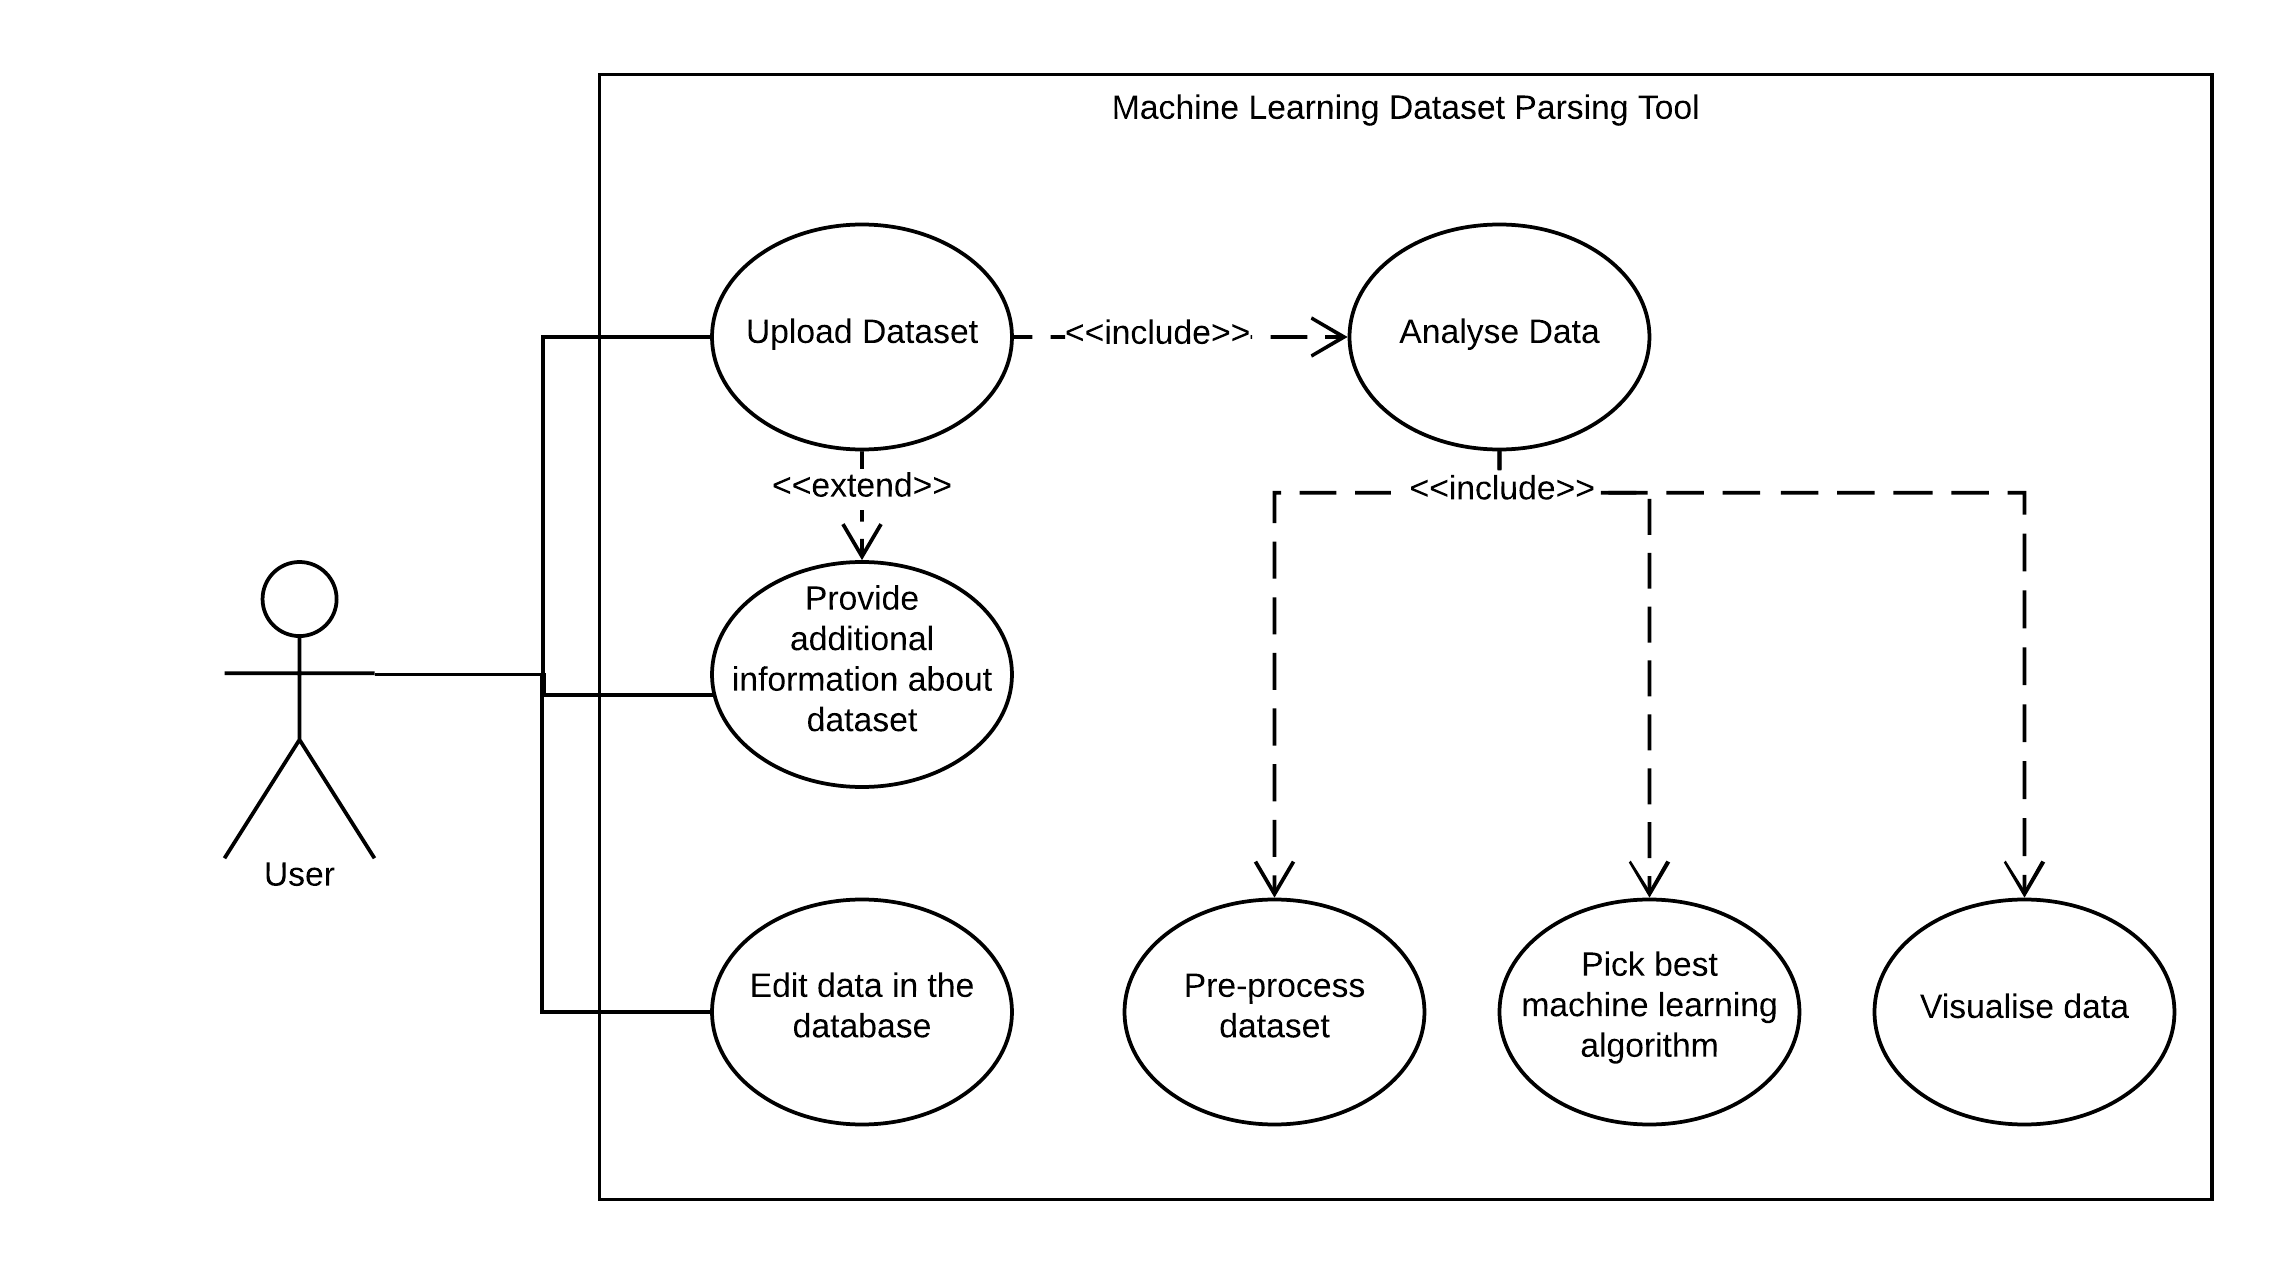
\includegraphics[width=\textwidth]{usecase}
  \caption{Simple use case diagram of the system}
  \label{usecase}
\end{figure}

The use case diagram clearly shows how the user will interact with the system. Due to the nature of the system, much of its complexity is hidden from the user and therefore the user does not have many use cases. Regardless, the use case diagram is an important part of the requirements gathering process as it makes it easier for the client to visualise their interactions with the system.

\section{Initial Design Ideas}
\section{Key Implementation Decisions}
\subsection{Database Design}

\subsubsection{NoSQL vs SQL}
Heterogenous big data benefits from NoSQL for a few reasons. Firstly, there is no predefined schema that the data has to conform to, which is useful for our application as we have to save data from a multitude of different data sources in the same data store. We cannot index all the data efficiently beforehand, and therefore cannot define a large schema that all datasets will conform to. Even if we could, a large schema would waste a lot of space, as most datasets would only use a small subset of the schema. This would also make searching the database very inefficient, as we would have to search through potentially hundreds of unused fields.

Removing schemas also makes the database faster to query \cite{sqlvsnosql}. Because each dataset is stored in one document rather than spread across multiple tables, the program knows exactly where to look for the data set rather than having to search through multiple tables. This helps when we are having to search through hundred of datasets to find the data set we are interested in.

\subsubsection{Lack of Relations Between Datasets}
The data sets that our program will use contain almost no relations. As such, using a relational database would waste a lot of the functionality associated with relations, and cause a lot of uneccessary overhead. Instead, a non-relational database will just store data sets independently of each other. Querying the database will simply involve returning a JSON object, with no links to other data sets.

\subsection{Accepted File Types in the System}

When studying Weka, the team found that there are many file types that machine learning tools could use, for instance Arff data files, CSV data files, XRFF data files, amongst others. After some research into the UCI Machine Learning Repository \cite{uci}, the team decided to use CSV data files to store datasets into the database and to be used by the machine learning tools. This is because CSV files make it convenient for the team to transform the .data files and .name files found on the UCI repository into a single file. CSV files are also easy to store in the NoSQL database. Knowing the format of the data is useful for data pre-processing and analysing.


\section{Problems Encountered}

\section{Time Planning and Project Management}
At the very start of the project, time planning was discussed but was not followed or enforced as much as it should have been. As such, a Gantt Chart was devised and is shown in figure \ref{ganttchart}. This Gantt chart has helped us stick to deadlines and structure our work.

\begin{figure}\label{ganttchart}
  
\end{figure}

Alongside the Gantt chart, we have a Kanban board which is hosted on Trello.com. Scrum was discussed as an alternative approach, but Kanban was chosen for some reasons outlined below:

\begin{itemize}
% \item For a little team like ours which has only 5 members, agile provides a more suitable framework for software development.
\item Teams using Kanban can cope with mutable requirements flexibly. Teamwork will continue with changing project environment.
\item Formal and informal meetings can be held as frequently as needed and agile working process can be pushed favorably by team communication.
\item Due to the main process of the project having been decided, Kanban is a good system as it allows us to vizualise every stage of work and everyone’s processing.
\item For a team with less development experience, it is difficult to deliver an executable program in a short time. Scrum would be difficult to practice because of its demand on techniques and experience.
\item Scrum need to stipulate working time for every iteration, which is difficult for teams with less development experience. Kanban only displays stage missions but not time limits.
\item Scrum needs to declare a Product Owner, Scrum manager and Team which might cause confusion in an inexperienced team. Kanban can make team members focus on their work and research.
\end{itemize}

\pagebreak
\bibliography{bibliography}{}
\bibliographystyle{IEEEtranN} 

\end{document}